\documentclass[12pt,british]{beamer}
\usetheme{focus}
\usepackage{graphicx}
\usepackage[british]{babel}
\usepackage{tikz}
\usetikzlibrary{arrows,backgrounds,decorations.pathmorphing,decorations,mindmap}

\title[DPoS]{Delegated Proof of Stake}
\author{Vladimir Komendantskiy}
\institute{POA Network}
\date{DLT-EDI // 28th February 2019}

\begin{document}

\pgfdeclareimage[height=2cm]{ETH}{icons8-ethereum-480}

\begin{frame}
  \maketitle
\end{frame}

\begin{frame}{Contents}
  \tableofcontents
\end{frame}

\section{Motivation}

\begin{frame}
  \frametitle{Idealised value transfer system}

  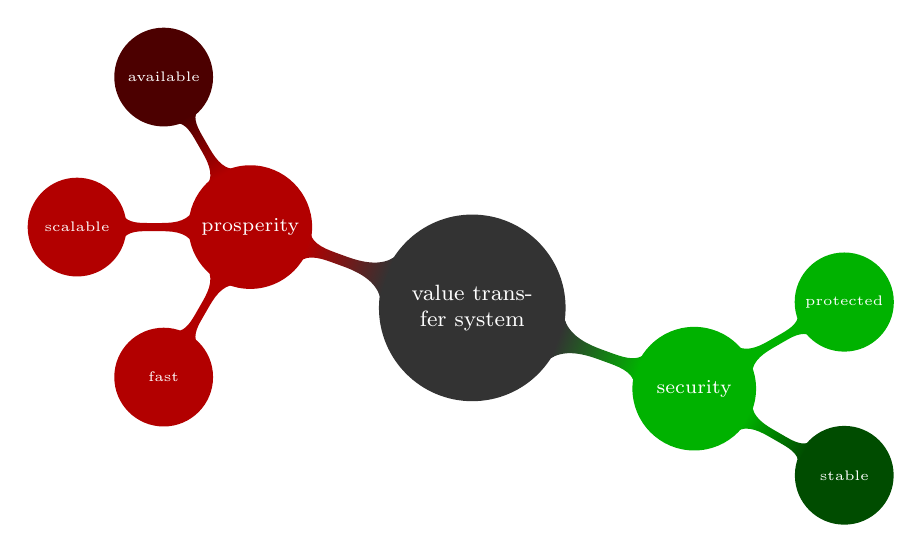
\begin{tikzpicture}
    [small mindmap,concept color=black!80,text=white,
      level 1/.append style={level distance=3cm,sibling angle=180},
      prosperity/.style={concept color=red!70!black,faded/.style={concept color=red!30!black}},
      security/.style={concept color=green!70!black,faded/.style={concept color=green!30!black}}
    ]

    \node [concept] {value transfer system}
          [clockwise from=160]
          child [prosperity] {node [concept] {prosperity}
            [clockwise from=240]
            child {node [concept] {fast}}
            child {node [concept] {scalable}}
            child [faded] {node [concept] {available}}
          }
          child [security] {node [concept] {security}
            [clockwise from=30]
            child {node [concept] {protected}}
            child [faded] {node [concept] {stable}}
          };
  \end{tikzpicture}
\end{frame}

\section{Definition}

\begin{frame}
  \frametitle{Delegated proof of stake consensus module}

  \begin{itemize}
  \item Provides economic incentive for honest and decentralised protocol
    execution.
  \item \emph{Validators} (block producers) are selected, or \emph{delegated},
    from participants.
  \item Participants can stake on
    \begin{itemize}
    \item themselves to get selected as a validator,
    \item others to get a share if and when they are selected.
    \end{itemize}
  \item Validators are chosen based on
    \begin{itemize}
    \item the amount at stake,
    \item a randomness beacon.
    \end{itemize}
  \end{itemize}
\end{frame}

\begin{frame}
  \frametitle{Incentives}

  \begin{itemize}
  \item \textbf{Honesty.} A node with malicious behaviour is reported and
    removed, and its stake confiscated.

  \item \textbf{Increased throughput.} Participants launch more consensus nodes
    (servers) to increase the probability of selection.

  \end{itemize}
\end{frame}

\begin{frame}
  \frametitle{Base consensus protocol: AuRa}

  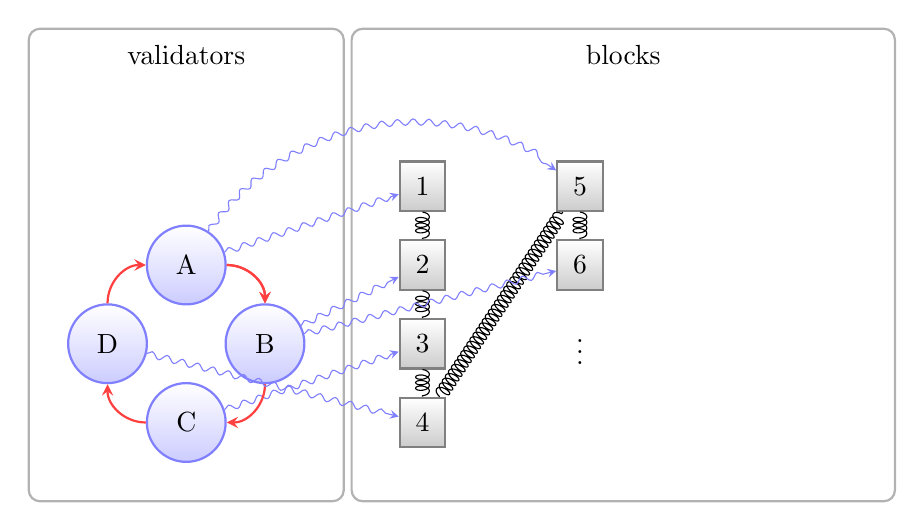
\begin{tikzpicture}
    [inner sep=2mm,
      collection/.style={draw=black!30,thick,rounded corners},
      validator/.style={circle,draw=blue!50,top color=white,bottom
        color=blue!20,thick,minimum height=1cm},
      block/.style={rectangle,draw=black!50,top color=white,bottom color=black!20,thick},
      mined/.style={-stealth,draw=blue!50,decorate,decoration=
        {snake,amplitude=.4mm,segment length=2mm,post length=1mm}
      },
      transition/.style={-stealth,thick,draw=red!75,bend angle=45},
      chain/.style={decorate,decoration={coil,segment length=2pt}}
    ]

    \begin{scope}[on background layer]
      \draw [collection] (-2,3)
      -- node [below,align=center,midway] {validators} (2,3)
      -- (2,-3) -- (-2,-3) -- cycle;
      \draw [collection] (2.1,3)
      -- node [below,align=center,midway] {blocks} (9,3)
      -- (9,-3) -- (2.1,-3) -- cycle;
    \end{scope}

    \node at ( 0, 0) [validator] (A) {A};
    \node at ( 1,-1) [validator] (B) {B};
    \node at ( 0,-2) [validator] (C) {C};
    \node at (-1,-1) [validator] (D) {D};

    \uncover<2-> {
      \node at (3, 1) [block] (b1) {1};
    }
    \uncover<2> {
      \draw [mined] (A) -- (b1);
    }
    \uncover<3-> {
      \node at (3, 0) [block] (b2) {2};
      \draw [chain] (b1) -- (b2);
    }
    \uncover<3> {
      \draw [mined] (B) -- (b2);
      \draw [transition] (A) to [bend left] (B);
    }
    \uncover<4-> {
      \node at (3,-1) [block] (b3) {3};
      \draw [chain] (b2) -- (b3);
    }
    \uncover<4> {
      \draw [mined] (C) -- (b3);
      \draw [transition] (B) to [bend left] (C);
    }
    \uncover<5-> {
      \node at (3,-2) [block] (b4) {4};
      \draw [chain] (b3) -- (b4);
    }
    \uncover<5> {
      \draw [mined] (D) -- (b4);
      \draw [transition] (C) to [bend left] (D);
    }
    \uncover<6-> {
      \node at (5, 1) [block] (b5) {5};
      \draw [chain] (b4) -- (b5);
    }
    \uncover<6> {
      \draw [mined] (A) to [bend left=45] (b5);
      \draw [transition] (D) to [bend left] (A);
    }
    \uncover<7-> {
      \node at (5, 0) [block] (b6) {6};
      \draw [chain] (b5) -- (b6);
    }
    \uncover<7> {
      \draw [mined] (B) -- (b6);
      \draw [transition] (A) to [bend left] (B);
      \node at (5,-1) {$\vdots$};
    }
  \end{tikzpicture}
\end{frame}

\begin{frame}
  \frametitle{Governance event: validator set change}

  \setbeamercovered{transparent}

  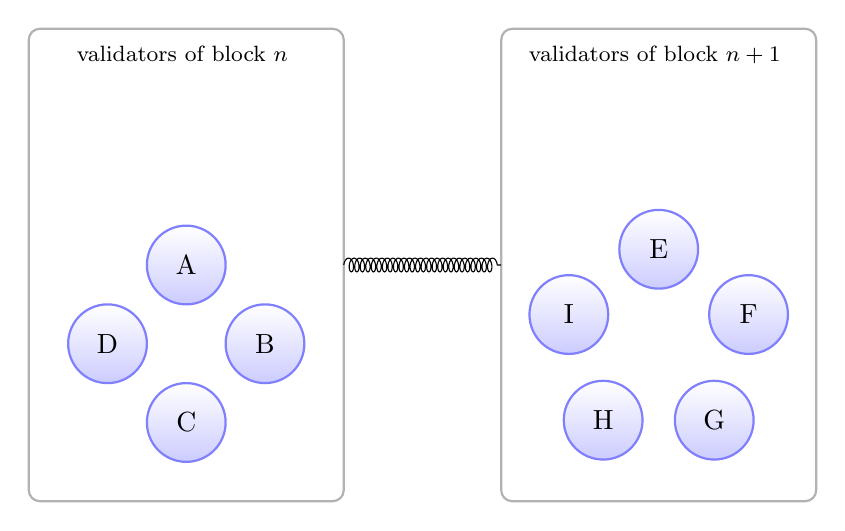
\begin{tikzpicture}
    [inner sep=2mm,
      collection/.style={draw=black!30,thick,rounded corners},
      validator/.style={circle,draw=blue!50,top color=white,bottom
        color=blue!20,thick,minimum height=1cm},
      chain/.style={decorate,decoration={coil,segment length=2pt}}
    ]

    \uncover<1> {
      \draw [collection] (-2,4)
      -- node [below,align=center,midway] {
        \footnotesize validators of block $n$
      } (2,4) -- node [left,align=center] (b1) {} (2,-2) -- (-2,-2) -- cycle;

      \node at ( 0, 1) [validator] (A) {A};
      \node at ( 1, 0) [validator] (B) {B};
      \node at ( 0,-1) [validator] (C) {C};
      \node at (-1, 0) [validator] (D) {D};
    }

    \uncover<2> {
      \draw [collection] (4,4)
      -- node [below,align=center,midway] {
        \footnotesize validators of block $n+1$
      } (8,4) -- (8,-2) -- (4,-2) -- node [right,align=center] (b2) {} cycle;

      \node at (90:1.2) [validator,xshift=6cm] (E) {E};
      \node at (18:1.2) [validator,xshift=6cm] (F) {F};
      \node at (-54:1.2) [validator,xshift=6cm] (G) {G};
      \node at (-126:1.2) [validator,xshift=6cm] (H) {H};
      \node at (-198:1.2) [validator,xshift=6cm] (I) {I};

      \draw [chain] (b1) -- (b2);
    }
  \end{tikzpicture}

  \setbeamercovered{invisible}

\end{frame}

\begin{frame}
  \frametitle{Participants (stakeholders)}

  \begin{tikzpicture}
    [inner sep=2mm,
      collection/.style={draw=black!30,thick,rounded corners},
      validator/.style={circle,draw=blue!50,top color=white,bottom
        color=blue!20,thick,minimum height=1cm},
      flow/.style={-stealth,shorten <=3pt,thick,dashed,draw=black!50,bend angle=60},
    ]

    \filldraw [collection,fill=green!10] (-2.5,5)
    -- node [below,align=center,midway] (delegators) {
      \footnotesize delegators
    } (9,5) -- (9,-2.5) -- (-2.5,-2.5) -- cycle;

    \node at (7.5,3) {\pgfuseimage{ETH}};

    \draw [collection,fill=orange!10] (-2.25,4)
    -- node [below,align=center,midway] (candidates) {
      \footnotesize candidates
    } (6,4) -- (6,-2.25) -- (-2.25,-2.25) -- cycle;

    \node at (90:1.2) [validator,xshift=4cm] (E) {E};
    \node at (18:1.2) [validator,xshift=4cm] (F) {F};
    \node at (-54:1.2) [validator,xshift=4cm] (G) {G};
    \node at (-126:1.2) [validator,xshift=4cm] (H) {H};
    \node at (-198:1.2) [validator,xshift=4cm] (I) {I};

    \draw [collection,fill=red!10] (-2,3)
    -- node [below,align=center,midway] (validators) {
      \footnotesize validators
    } (2,3) -- (2,-2) -- (-2,-2) -- cycle;

    \node at ( 0, 1) [validator] (A) {A};
    \node at ( 1, 0) [validator] (B) {B};
    \node at ( 0,-1) [validator] (C) {C};
    \node at (-1, 0) [validator] (D) {D};

    \pause

    \draw [flow] (delegators.east)
    to [bend left] node [midway,right] {\tiny stakes} (candidates.east);

    \draw [flow] (candidates.east)
    to [bend left] node [midway,right] {\tiny selection} (validators.east);
  \end{tikzpicture}
\end{frame}

\begin{frame}
  \frametitle{Participant transitions}

  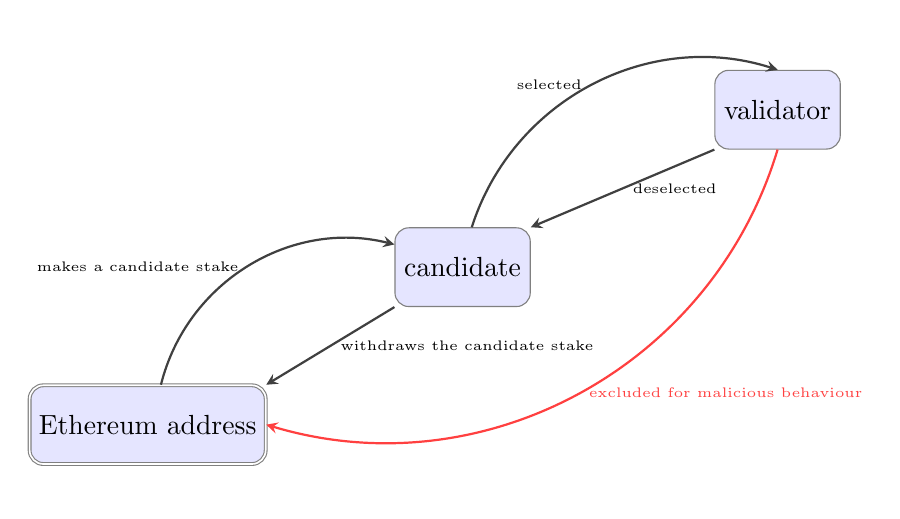
\begin{tikzpicture}
    [
      -stealth,
      state/.style={draw=black!50,fill=blue!10,rectangle,rounded corners=5pt,
        minimum height=1cm},
      transition/.style={-stealth,thick,draw=black!75}
    ]

    \node at (0,0) [state,double] (address) {Ethereum address};
    \node at (4,2) [state] (candidate) {candidate};
    \node at (8,4) [state] (validator) {validator};

    \draw [transition] (address) to [bend left=45] node [midway,left] {
      \tiny makes a candidate stake
    } (candidate);

    \draw [transition] (candidate.south west) to node [midway,right] {
      \tiny withdraws the candidate stake
    } (address.north east);

    \draw [transition] (candidate) to [bend left=45] node [midway,left] {
      \tiny selected
    } (validator.north);

    \draw [transition] (validator.south west) to node [midway,right] {
      \tiny deselected
    } (candidate.north east);

    \draw [transition,draw=red!75] (validator.south) to [bend left=45]
    node [midway,right,red!75] {\tiny excluded for malicious behaviour}
    (address.east);
  \end{tikzpicture}
\end{frame}

\section{Rules}

\begin{frame}[fragile]
  \frametitle{Genesis}

  \alert{Addresses} contained in the genesis block:
  \begin{itemize}
  \item governance contract owner
  \item initial validators
  \end{itemize}

  ... and DPoS \alert{parameters}:
  \begin{itemize}
  \item \verb|MAX_CANDIDATES|
  \item \verb|MAX_VALIDATORS|
  \item \verb|CANDIDATE_MIN_STAKE|
  \item \verb|DELEGATOR_MIN_STAKE|
  \item \verb|STAKING_EPOCH_PERIOD|
  \end{itemize}
\end{frame}

\begin{frame}
  \frametitle{Staking epoch}

  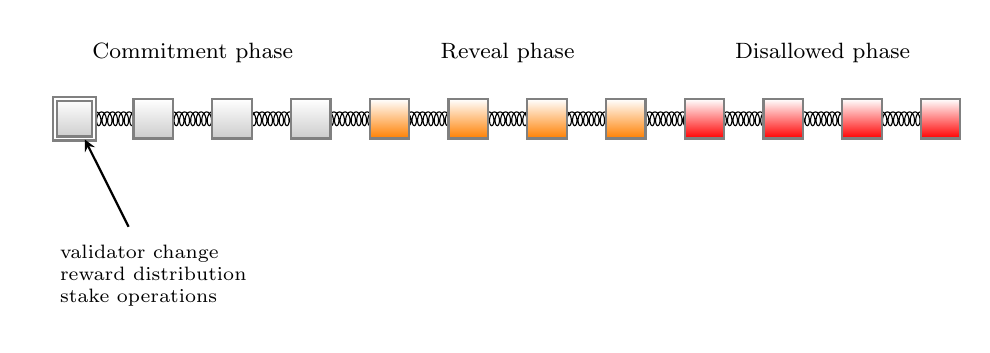
\begin{tikzpicture}
    [inner sep=2mm,
      block/.style={rectangle,minimum width=0.5cm,minimum height=0.5cm,
        draw=black!50,top color=white,bottom color=black!20,thick},
      chain/.style={decorate,decoration={coil,segment length=2pt}}
    ]
    \draw [chain]
    (0,0) node [block,double] (cStart) {} --
    (1,0) node [block] {} --
    (2,0) node [block] {} --
    (3,0) node [block] (cEnd) {} --
    (4,0) node [block,bottom color=orange] (rStart) {} --
    (5,0) node [block,bottom color=orange] {} --
    (6,0) node [block,bottom color=orange] {} --
    (7,0) node [block,bottom color=orange] (rEnd) {} --
    (8,0) node [block,bottom color=red] (dStart) {} --
    (9,0) node [block,bottom color=red] {} --
    (10,0) node [block,bottom color=red] {} --
    (11,0) node [block,bottom color=red] (dEnd) {};

    \path (cStart) -- node [above=0.5cm] {\footnotesize Commitment phase} (cEnd);
    \path (rStart) -- node [above=0.5cm] {\footnotesize Reveal phase} (rEnd);
    \path (dStart) -- node [above=0.5cm] {\footnotesize Disallowed phase}
    (dEnd);

    \node at (1,-2) (note) {
      \scriptsize
      \begin{tabular}{l}
        validator change\\
        reward distribution\\
        stake operations
      \end{tabular}
    };

    \draw [thick,-stealth] (note) -- (cStart);
  \end{tikzpicture}
\end{frame}

\begin{frame}
  \frametitle{Validator selection}

  Starting from the second epoch, validators are determined by
  \begin{itemize}
    \item the distributed randomness of the previous staking
      epoch,
    \item the amount at stake for each candidate validator,
    \item extra tuning parameters of the economic model.
  \end{itemize}
\end{frame}

\begin{frame}
  \frametitle{Randomness beacon}

  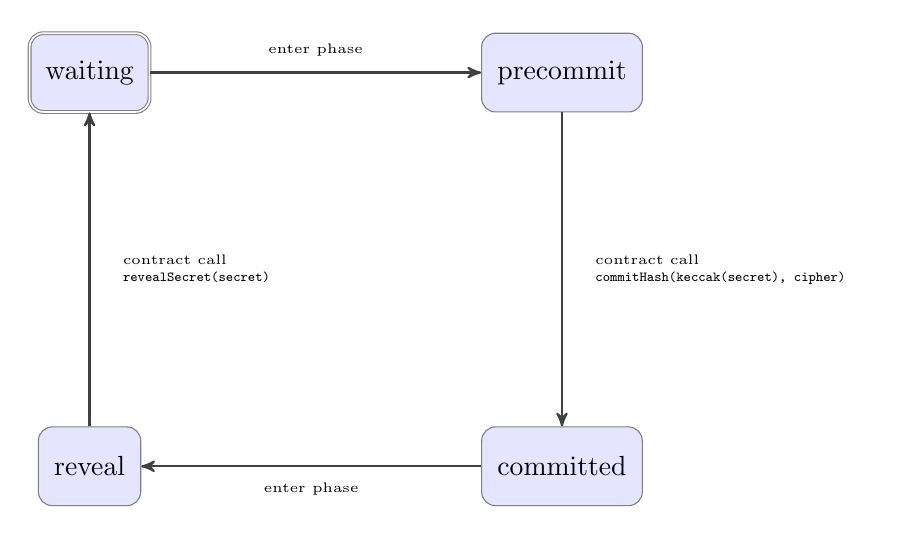
\begin{tikzpicture}
    [
      inner sep=2mm,
      state/.style={draw=black!50,fill=blue!10,rectangle,rounded corners=5pt,
        minimum height=1cm},
      transition/.style={-stealth',thick,draw=black!75}
    ]

    \node at (0,0) [state,double] (waiting) {waiting};
    \node at (6,0) [state] (precommit) {precommit};
    \node at (6,-5) [state] (committed) {committed};
    \node at (0,-5) [state] (reveal) {reveal};

    \draw [transition] (waiting) -- node [above] {\tiny enter phase} (precommit);
    \draw [transition] (precommit) -- node [right] {
      \tiny
      \begin{tabular}{l}
        contract call \\
        \mbox{\texttt{commitHash(keccak(secret), cipher)}}
      \end{tabular}
    } (committed);
    \draw [transition] (committed) -- node [below] {\tiny enter phase} (reveal);
    \draw [transition] (reveal) -- node [right] {
      \tiny
      \begin{tabular}{l}
        contract call \\
        \mbox{\texttt{revealSecret(secret)}}
      \end{tabular}
    } (waiting);
  \end{tikzpicture}
\end{frame}

\begin{frame}
  \frametitle{Further references}

  \begin{enumerate}
  \item POA Network DPoS whitepaper (upcoming, 2019)
  \item DPoS DAO Solidity contracts: {\footnotesize
    \url{https://github.com/poanetwork/posdao-contracts}}
  \item These slides: {\footnotesize
    \url{https://github.com/vkomenda/dlt-edi-2019-02-28}}
  \item Voting software: \url{https://xkcd.com/2030/}
  \end{enumerate}

\end{frame}

\begin{frame}
  \frametitle{Ask the engineer}

  \centering {
    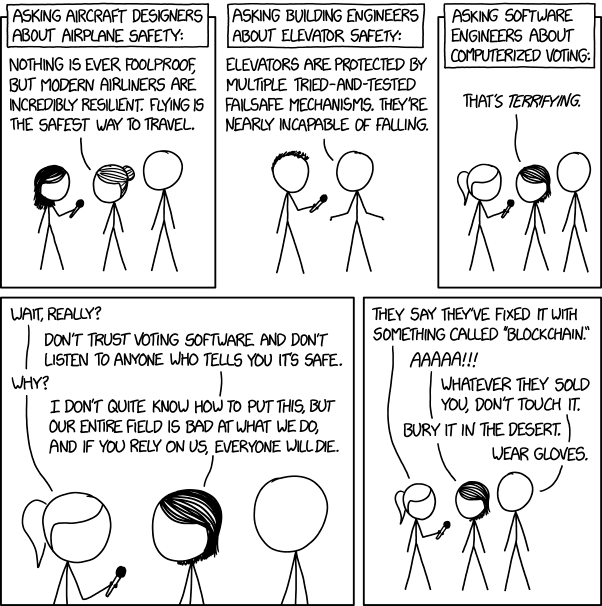
\includegraphics[height=7cm]{voting_software.png}
  }
\end{frame}

\end{document}
